\documentclass[a4paper, 7pt, landscape]{scrartcl}
\usepackage[german]{babel}
\usepackage[utf8]{inputenc}
\usepackage{multicol}
\usepackage{geometry}
\usepackage{graphicx}
\usepackage{wrapfig}
\usepackage{enumitem}
\usepackage{fancyhdr}
\usepackage{index}
\usepackage{sectsty}
\usepackage{mwe}
\usepackage{comment}
\usepackage{lipsum}
\usepackage{titlesec}
\usepackage[dvipsnames]{xcolor}
\usepackage{amsmath}
\usepackage{amssymb}
\usepackage{listings}

%Define Math Commands:
\newcommand*{\field}[1]{\mathbb{#1}}%
\newcommand{\Mod}[1]{\ (\mathrm{mod}\ #1)}

%Image Folder:
\graphicspath{{../img/}}

%format
\geometry{top=0.4cm,left=0.5cm,right=0.5cm,bottom=0.4cm}
\setlist{topsep=0pt, leftmargin=5mm, nolistsep}

% Code Snippets

\definecolor{javared}{rgb}{0.6,0,0} % for strings

\lstset{
language=C,
basicstyle=\fontsize{7}{7} \ttfamily,
keywordstyle=\bfseries\color{RoyalBlue},
stringstyle=\color{javared},
commentstyle=\color{MidnightBlue},
morecomment=[s][\color{MidnightBlue}]{/**}{*/},
tabsize=2,
showspaces=false,
showstringspaces=false,
texcl = true,
rulecolor = \color{black},
breaklines = true,
aboveskip = 0em,
belowskip = 0em
}




% Define Section Format
\titleformat{name=\section}[block]
{\sffamily\normalsize}
{}
{0pt}
{\colorsection}
\titlespacing*{\section}{0pt}{0pt}{0pt}

\newcommand{\colorsection}[1]{%
\colorbox{MidnightBlue!40}{\parbox{0.98\linewidth}{\color{black}\thesection\ #1}}}


% Define Subsection Format
\titleformat{name=\subsection}[block]
{\sffamily\small}
{}
{0pt}
{\colorsubsection}
\titlespacing*{\subsection}{0pt}{0pt}{0pt}

\newcommand{\colorsubsection}[1]{%
\colorbox{YellowGreen!50}{\parbox{0.98\linewidth}{\color{black}\thesubsection\ #1}}}

% Define SubSubsection Format
\titleformat{name=\subsubsection}[block]
{\sffamily\small}
{}
{0pt}
{\colorsubsubsection}
\titlespacing*{\subsubsection}{0pt}{0pt}{0pt}

\newcommand{\colorsubsubsection}[1]{%
\colorbox{Goldenrod!50}{\parbox{0.98\linewidth}{\color{black}\thesubsubsection\ #1}}}

% -----------------------------------------------------------------------
\begin{document}
    %	\pagecolor{p}
    %	\color{t}
    \setlength{\columnseprule}{0.4pt}
    \footnotesize
    \begin{multicols*}{3}

        %! Author = Philipp Emmenegger
%! Date = 30/06/2021

\section{Introduction}
\subsection{Pattern Definition}
\begin{itemize}
    \item Descriptions of successful engineering stories
    \item Address recurring problem
    \item Descripe generic solution that worked
    \item Tell about the forces of the problem (why is the problem hard)
    \item Tell about the engineering trade-offs  to take (Benefits / Liabilities)
    \item Solution (Implementation)
\end{itemize}

\subsection{Type of Patterns}
\begin{itemize}
    \item Architecture Patterns (Waiting Room)
    \item Software Patterns
    \begin{itemize}
        \item Design Pattern (Elements of Reusable Object-Oriented Sofware)
        \item Pattern-oriented Software Architecture (POSA)
    \end{itemize}
    \item Organizational Patterns
    \item Learning and Teaching Patterns
    \item Documentation Patterns
\end{itemize}

\subsection{Pattern Formats}
\subsubsection{POSA}
\begin{itemize}
    \item Pattern name
    \item Intent
    \item Problem
    \item Solution
    \item Benefits / Liabilities
\end{itemize}
\subsubsection{Fault Tolerance}
\begin{itemize}
    \item Name
    \item Intent
    \item Solution
    \item Benefits / Liabilities
\end{itemize}
\subsubsection{MAPI}
\begin{itemize}
    \item Name
    \item Intent
    \item Consequences
\end{itemize}
\subsubsection{Game Programming Patterns}
\begin{itemize}
    \item Name
    \item Problem
    \item Engineering Story that worked
    \item Benefits / Liabilities
    \item Solution
\end{itemize}

\subsection{What are Patterns not?}
\begin{itemize}
    \item Silver bullet
    \item Novices Tool
    \item Ready Made Components
    \item Means to turn off your brain
\end{itemize}

        \section{GoF Patterns}
\subsection{Observer}
Define a one-to-many dependency between objects so that when one object changes state, all its dependents are notified and updated automatically.\\
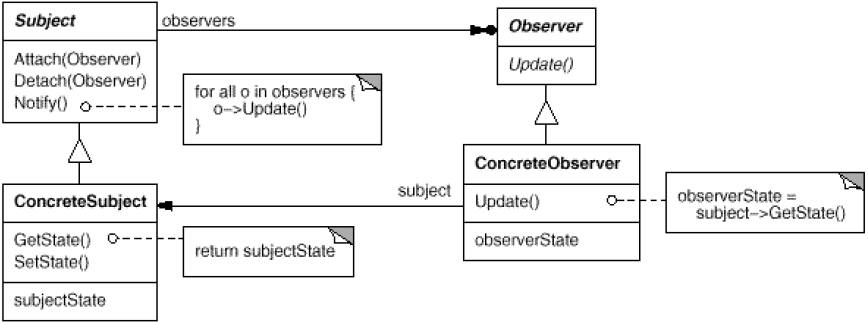
\includegraphics[width=\linewidth]{./img/observer.png}

\subsection{Strategy}
Define a family of algorithms, encapsulate each one, and make them interchangeable. Strategy lets the algorithm vary independently from clients that use it.\\
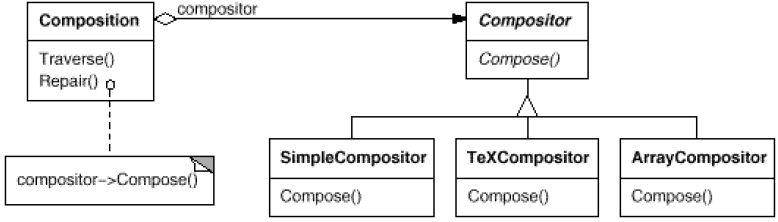
\includegraphics[width=\linewidth]{./img/strategy.png}

\subsection{Template Method}
Define the skeleton of an algorithm in an operation, deferring some steps to subclasses. Template Method lets subclasses redefine certain steps of an algorithm without changing the algorithm's structure.\\
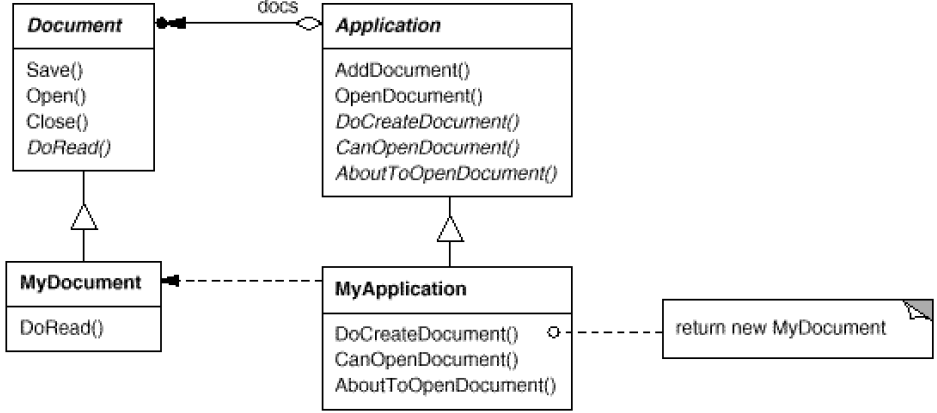
\includegraphics[width=\linewidth]{./img/template_method.png}

\subsection{Factory Method}
Define an interface for creating an object, but let the subclass decide which class to instantiate. Factory Method lets a class defer instantiation to subclasses.\\
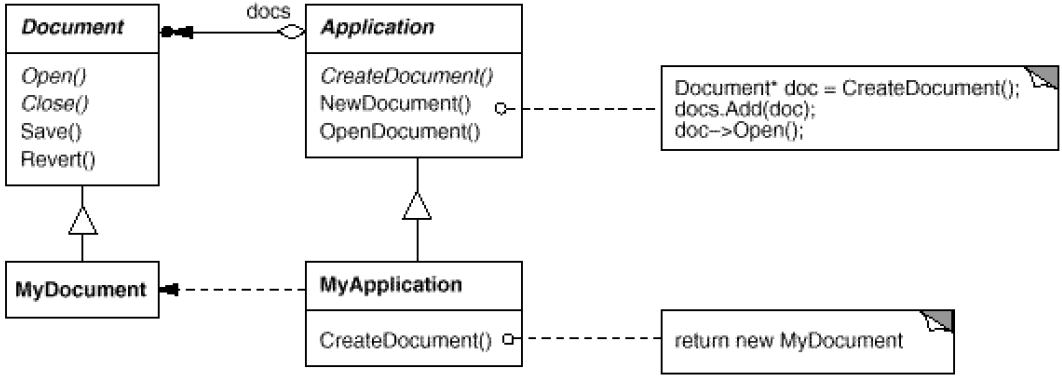
\includegraphics[width=\linewidth]{./img/factory_method.png}

\subsection{Abstract Factory}
Provide an interface for creating families of related or dependant objects without specifying their concrete classes.\\ 
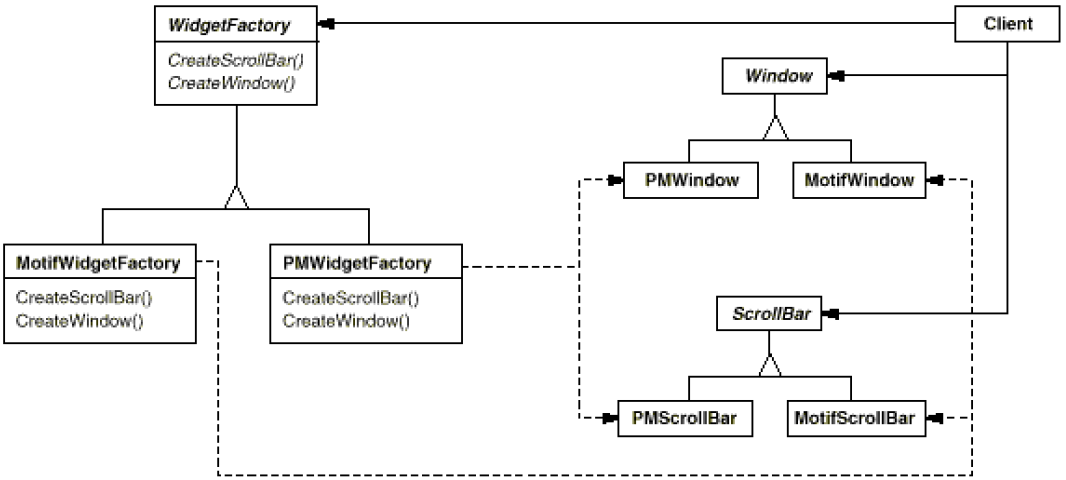
\includegraphics[width=\linewidth]{./img/abstract_factory.png}

\subsection{Prototype}
Specify the kinds of objects to create using a prototypical instance, and create new objects by copying this prototype.\\ 
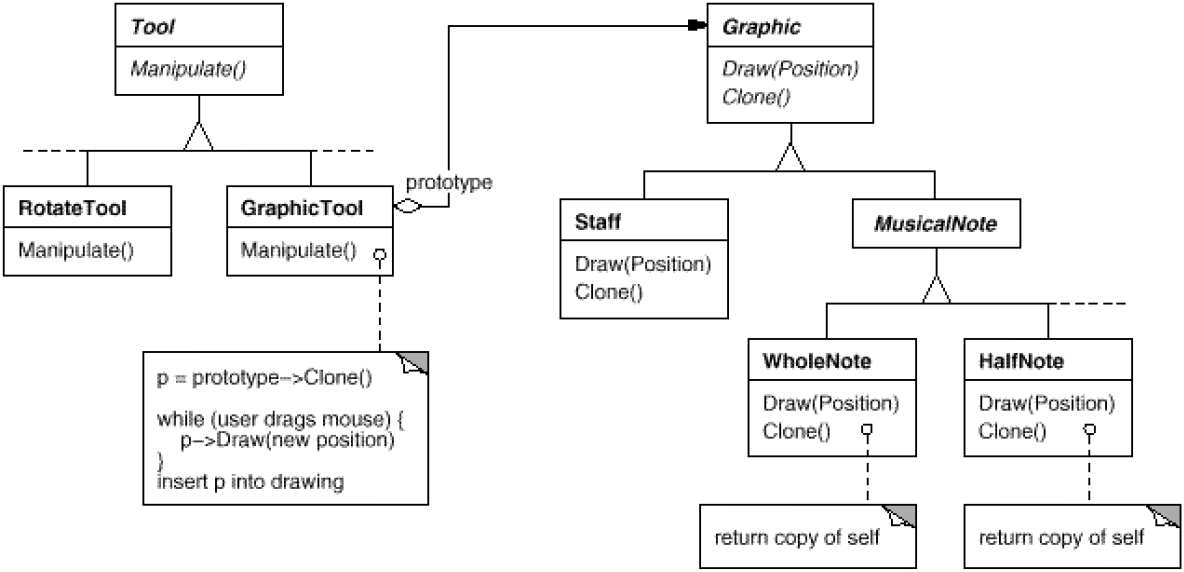
\includegraphics[width=\linewidth]{./img/prototype.png}

\subsection{Composite}
Compose objects into tree structures to represent part-whole hierarchies. Composite lets clients treat individual objects and compositions of objects uniformly.\\ 
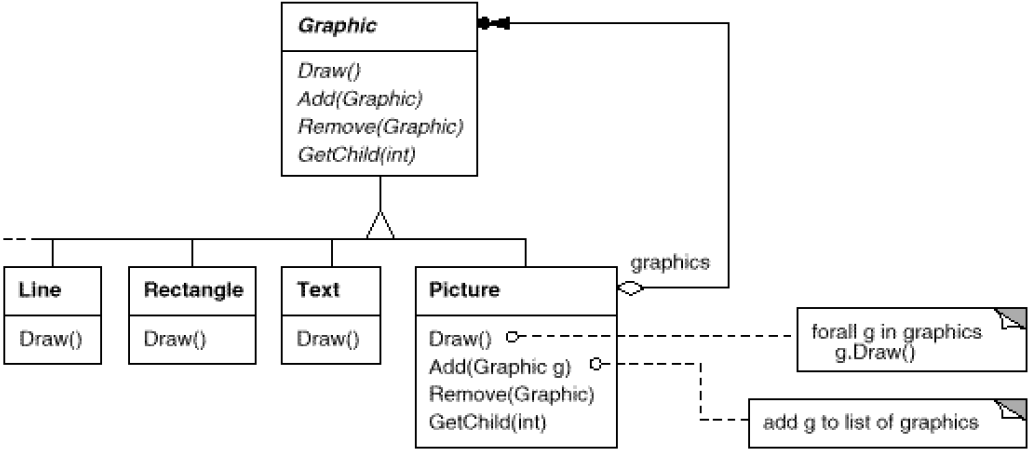
\includegraphics[width=\linewidth]{./img/composite.png}


\subsection{Decorator}
Attach additional responsibilities to an object dynamically. Decorators provide a flexible alternative to subclassing for extending functionality.\\ 
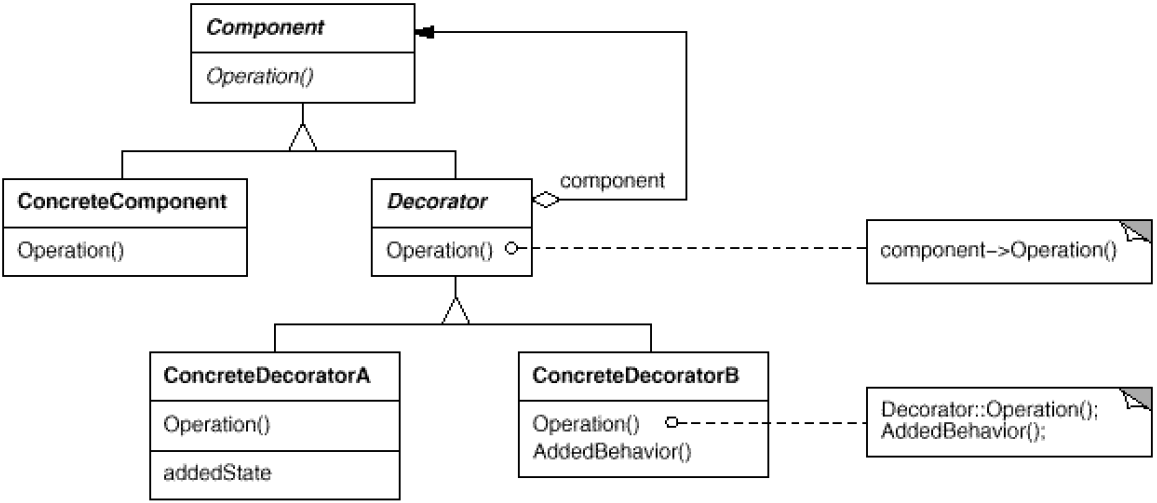
\includegraphics[width=\linewidth]{./img/decorator.png}

\subsection{Adapter}
Convert the interface of a class into another interface clients expect. Adapter lets classes work together that couldn't otherwise because of incompatible interfaces.\\ 
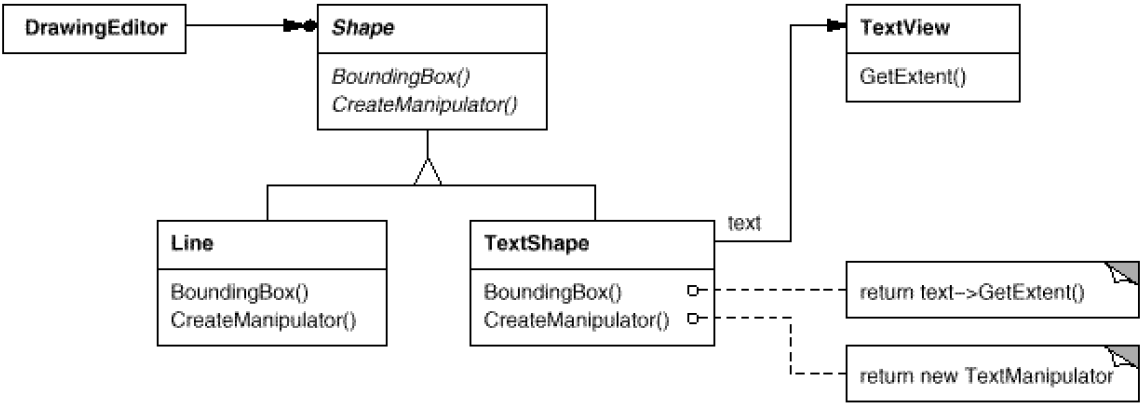
\includegraphics[width=\linewidth]{./img/adapter.png}

\subsection{Proxy}
Provide a surrogate or placeholder for another object to control access to it.\\ 
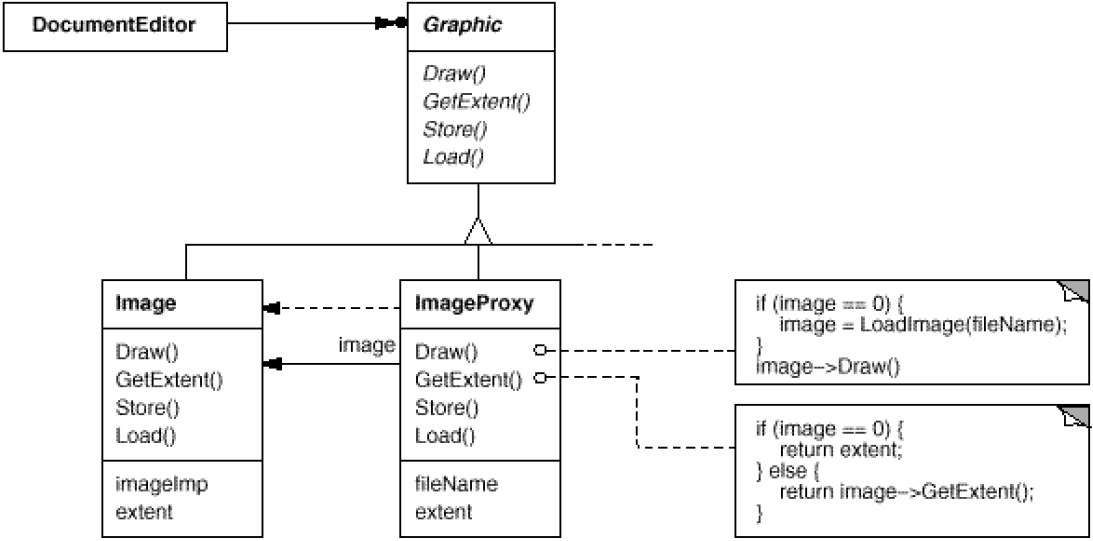
\includegraphics[width=\linewidth]{./img/proxy.png}

\subsection{Facade}
Provide a unified interface to a set of interfaces in a subsystem. Facade defines a higher-level interface that makes the subsystem easier to use.\\ 
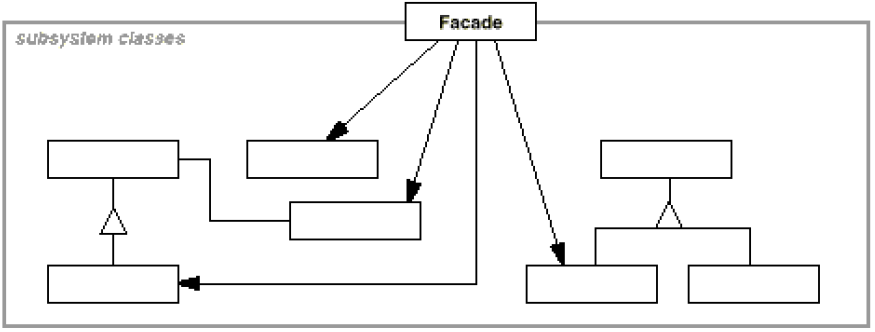
\includegraphics[width=\linewidth]{./img/facade.png}

\subsection{Mediator}
\subsubsection{Problem}
\begin{itemize}
    \item Object Structures may result in many connections between objects
    \item In the worst case, every object ends up knowing about every other
\end{itemize}
\textbf{Intent:}
\begin{itemize}
    \item How can strong coupling between multiple objects be avoided and communication simplified?
\end{itemize}
\subsubsection{Solution}
Define an object that encapsulates how a set of objects interact. Mediator promotes loose coupling by keeping objects from referring to each other explicitly, and lets you vary their interaction independently.\\ 
\textbf{Mediator:} Encapsulates how a set of objects interact\\ 
\textbf{Colleaues:} Refer to Mediator; this promotes loose coupling\\ 
\textbf{Static Structure:}\\
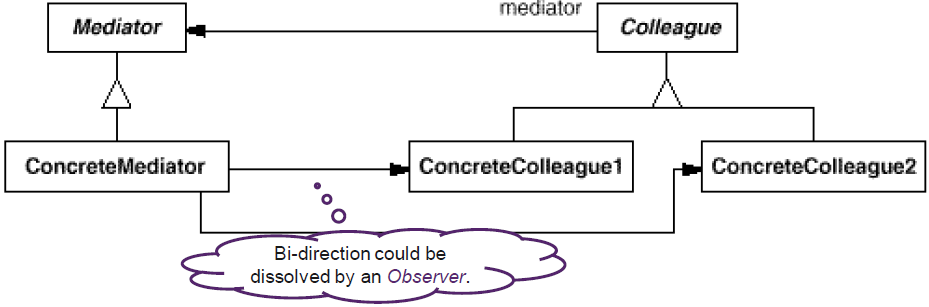
\includegraphics[width=\linewidth]{./img/mediator_static.png}
\textbf{Dynamics:}\\ 
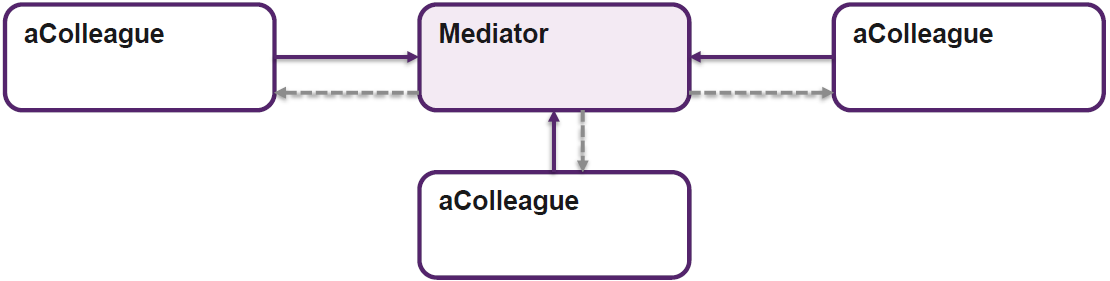
\includegraphics[width=\linewidth]{./img/mediator_dynamic.png}
\subsubsection{Implementation}
\begin{itemize}
    \item Mediator as an Observer
    \item Colleagues act as Subject
\end{itemize}
\textbf{Known Uses:}
\begin{itemize}
    \item Message Bus Systems
    \item Redux Dispatcher
\end{itemize}
\subsubsection{Summary}
\textbf{Benefits:}
\begin{itemize}
    \item Colleague classes may become more reusable, low coupling
    \item Centralizes control of communication between objects
    \item Encapsulates protocols
\end{itemize}
\textbf{Liabilities:}
\begin{itemize}
    \item Adds complexity
    \item Single point of failure
    \item Limits subclassing (of mediator class)
    \item May result in hard maintainable monoliths
\end{itemize}

\subsection{Memento}
\subsubsection{Problem}
\begin{itemize}
    \item Sometimes it's necessary to record the internal state of an object
    \item Objects normally encapsulate their state, making it inaccessible
\end{itemize}
\textbf{Intent:}
\begin{itemize}
    \item How can the state of an object be externalized without violating its encapsulation?
\end{itemize}
\subsubsection{Solution}
Without violating encapsulation, capture and externalize an objects internal state so that the object can be restored to this state later.\\
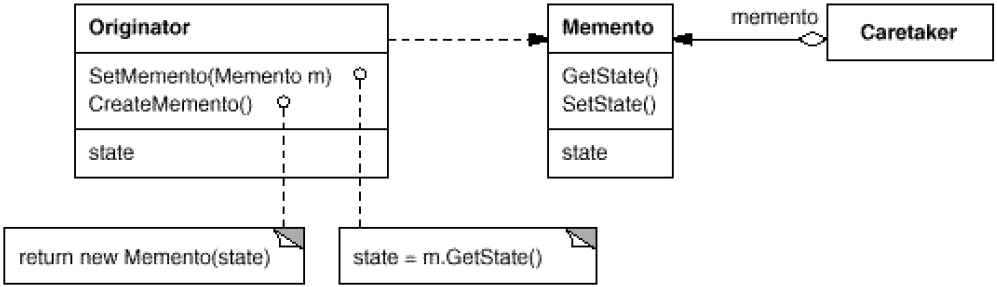
\includegraphics[width=\linewidth]{./img/memento.png}
\textbf{Dynamics:}\\ 
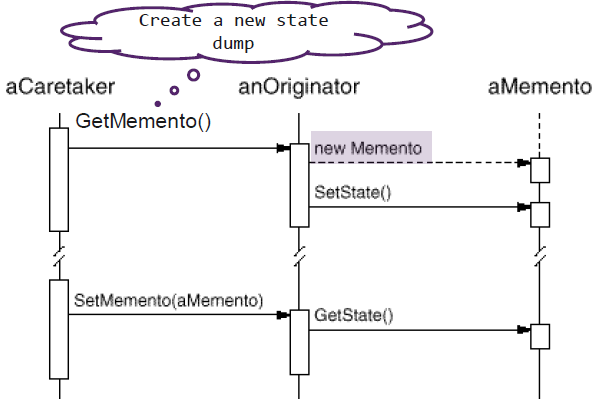
\includegraphics[width=0.7\linewidth]{./img/memento_dynamic.png}

\subsubsection{Participants}
\textbf{Memento}
\begin{itemize}
    \item Stores some / all the internal state of the Originator
    \item Allows only the originator to access its internal information
\end{itemize}
\textbf{Originator}
\begin{itemize}
    \item Can create Memento objects to store its internal state at strategic points
    \item Can restore own state to what the Memento object dictates
\end{itemize}
\textbf{Caretaker}
\begin{itemize}
    \item Stores the Memento objects
    \item Cannot explore / operate the contents 
\end{itemize}
\subsubsection{Implementation}
\begin{itemize}
    \item Originator creates memento and passes over its internal state
    \item Can be combined with Factory Method
    \item Declare Originator as \textit{friend} of Memento, so Originator can read out its properties
\end{itemize}
\subsubsection{Summary}
\textbf{Benefits}
\begin{itemize}
    \item Internal State of an object can be saved and restored at any time
    \item Encapsulation of attributes is not harmed
    \item State of objects can be restored later
\end{itemize}
\textbf{Liabilities}
\begin{itemize}
    \item Creates a complete copy of the object every time, no diffs (memory usage)
    \item No direct access to saved state, it must be restored first
\end{itemize}


\subsection{Command}
\subsubsection{Problem}
\begin{itemize}
    \item Decouple the decision of what to execute from the decision of when to execute
    \item The execution needs an additional parametrization context
\end{itemize}
\textbf{Intent:}
\begin{itemize}
    \item How can commands be encapsulated, so that they can be parameterized, scheduled, logged and/or undone?
\end{itemize}
\subsubsection{Solution}
Encapsulate a request as an object, thereby letting you parameterize clients with different requests, queue or log requests, and support undoable operation.\\ 
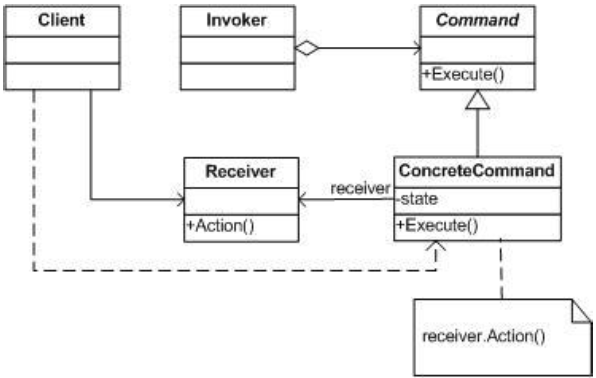
\includegraphics[width=\linewidth]{./img/command.png}
\textbf{Dynamics:}\\ 
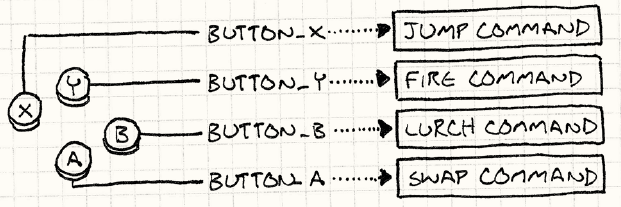
\includegraphics[width=\linewidth]{./img/command_dynamic.png}
\subsubsection{Summary}
\textbf{Benefits:}
\begin{itemize}
    \item The same command can be activated from different objects
    \item New commands can be introduced quickly and easily
    \item Command objects can be saved in a command history
    \item Provides inversion of control, encourages decoupling in both time and space
\end{itemize}
\textbf{Liabilities:}
\begin{itemize}
    \item Large designs with many commands can introduce many small command classes mauling the design
\end{itemize}

\subsection{Command Processor}
\subsubsection{Problem}
\begin{itemize}
    \item Common UI applications support do and multiple undo steps
    \item Steps forward and backward are accessible in a history
\end{itemize}
\textbf{Intent:}
\begin{itemize}
    \item How could we manage command objects, so the execution is seperated from the request and the execution can be undone later?
\end{itemize}
\subsubsection{Solution}
Separate the request for a service from its execution. A command processor component manages requests as separate objects, schedules their execution, and provides additional services such as the storing of request objects for later undo.\\ 
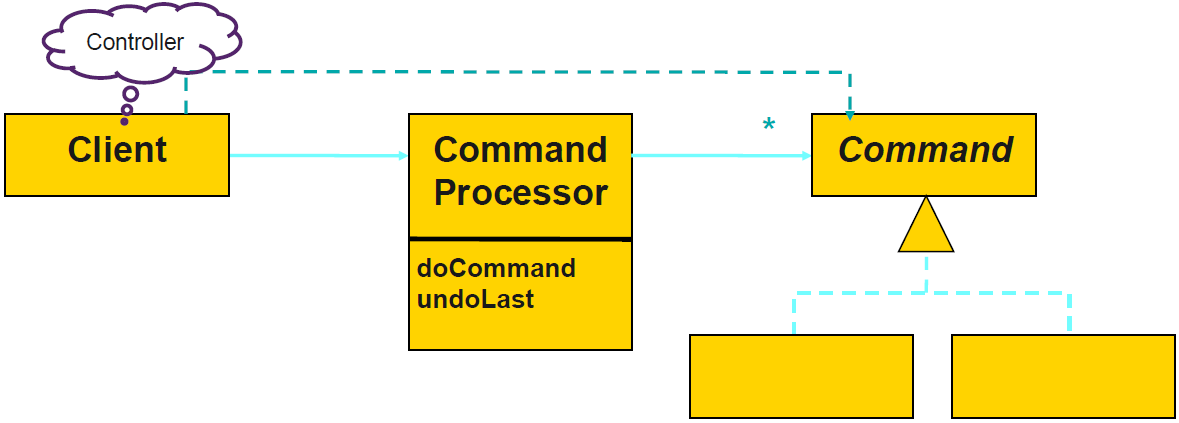
\includegraphics[width=0.8\linewidth]{./img/command_processor.png}
\textbf{Dynamics:}\\ 
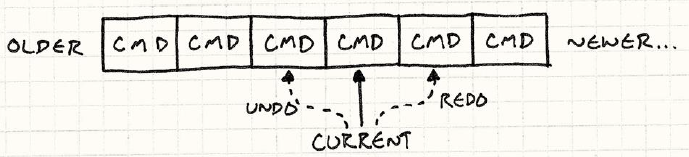
\includegraphics[width=\linewidth]{./img/command_processor_dynamic.png}
\subsubsection{Participants}
\textbf{Command Processor}
\begin{itemize}
    \item A Separate processor object can handle the responsibility for multiple Command objects
\end{itemize}
\textbf{Command}
\begin{itemize}
    \item A uniform interface to execute functions
\end{itemize}
\textbf{Controller}
\begin{itemize}
    \item Translates requests into commands and transfers commands to Command Processor.
\end{itemize}
\subsubsection{Implementation}
\begin{itemize}
    \item Command Processor contains a \textit{Stack} which holds the command history
    \item Controller creates the Commands and passes them over to Command Processor
    \item Creation of Commands may be delegated to a \textit{Simple Factory}
\end{itemize}
\subsubsection{Summary}
\textbf{Benefits:}
\begin{itemize}
    \item Flexibility
    \item Allows addition of services related to command execution
    \item Enhances testability
\end{itemize}
\textbf{Liabilities:}
\begin{itemize}
    \item Efficiency loss due additional indirection
\end{itemize}

\subsection{Visitor}
\subsubsection{Problem}
\begin{itemize}
    \item Operations on specific classes needs to be changed/added without needing to modify these classes
    \item Different algorithms needed to process an object tree
\end{itemize}
\textbf{Intent:}
\begin{itemize}
    \item How can the behaviour on individual elements of a data structure be changed/replaced whout changing the elements?
\end{itemize}
\subsubsection{Solution}
Represent an operation to be performed on the elements of an object structure. Visitor lets you define a new operation without changing the classes of the elements on which it operates.\\ 
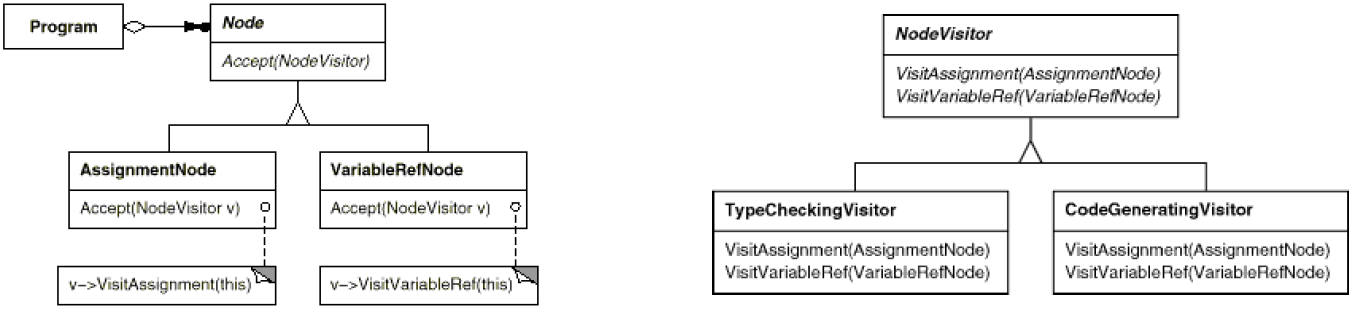
\includegraphics[width=\linewidth]{./img/visitor.png}
\subsubsection{Implementation}
\begin{itemize}
    \item 2 Class Hierarchies (Elements / Visitors)
    \item Visitors iterate though object hierarchy
    \item Solves Double-Dispatch problem of single dispatched programming languages
\end{itemize}
\textbf{Patterns that combine naturally with Vistor:}
\begin{itemize}
    \item Composite
    \item Interpreter
    \item Chain of Responsibility
\end{itemize}
\subsubsection{Summary}
\textbf{Benefits:}
\begin{itemize}
    \item Visitor makes adding new operatios easy
    \item Separates related operations from unrelated ones
\end{itemize}
\textbf{Liabilities:}
\begin{itemize}
    \item Adding new node classes is hard
    \item Visiting sequence fix defined within nodes
    \item Visitor breaks logic apart
\end{itemize}

        \section{Beyond GoF}
\subsection{External Iterator}
\subsubsection{Problem}
\begin{itemize}
    \item Iteration through a collection depends on the target implementation
    \item Separate logic of iteration into an object to allow multiple iteration strategies
\end{itemize}
\textbf{Intent:}
\begin{itemize}
    \item How can strong coupling between iteration and collection be avoided, generalized and provided in a collection-optimized manner?
\end{itemize}
\subsubsection{Solution}
Provide a way to access the elements of an aggregate object sequentially without exposing its underlying representation.\\ 
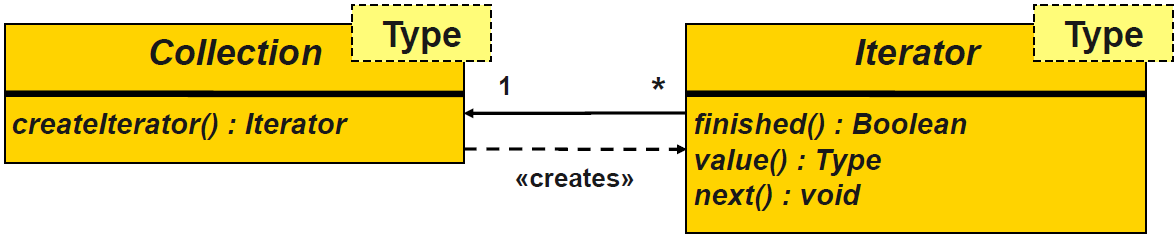
\includegraphics[width=\linewidth]{./img/external_iterator.png}
\textbf{Elementary operations of an Iterator's behaviour:}
\begin{itemize}
    \item Initializing an iteration \textit{new ArrayList().iterator();}
    \item Checking a completion condition \textit{it.hasNext();}
    \item Accessing a current target value \textit{var x = it.next();}
    \item Moving to the next target value \textit{it.next();}
\end{itemize}
\subsubsection{Summary}
\textbf{Benefits:}
\begin{itemize}
    \item Provides a single interface to loop though any kind of collection
\end{itemize}
\textbf{Liabilities:}
\begin{itemize}
    \item Multiple iterators may loop through a collection at the same time
    \item Life-Cycle Management of iterator objects
    \item Close coupling between Iterator and Collection class
    \item Indexing might be more intuitive for programmers
\end{itemize}

\subsection{Enumeration Method}
\subsubsection{Problem:}
\begin{itemize}
    \item Iteration management is performed by the collection's user
    \item Avoid state management between collection and iteration
\end{itemize}
\textbf{Intent:}
\begin{itemize}
    \item How can a collection be iterated considering the collection state and furthermore state management be reduced?
\end{itemize}
\subsubsection{Solution}
Support encapsulated iteration over a collection by placing responsibility for iteration in a method on the collection. The method takes a Command object that is applied to the elements of the collection.\\ 
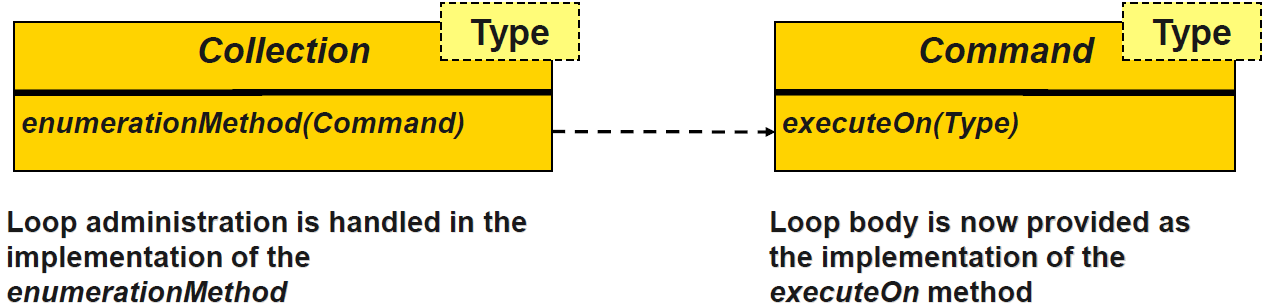
\includegraphics[width=\linewidth]{./img/enumeration_method.png}
\subsubsection{Summary}
Programming languages already implement Enumeration Method as their loop construct. (e.g. \textit{.forEach()})\\ 
\textbf{Benefits:}
\begin{itemize}
    \item Client is not responsible for loop housekeeping details
    \item Synchronization can be provided at the level of the whole traversal rather than for each element access
\end{itemize}
\textbf{Liabilities:}
\begin{itemize}
    \item Functional approach, more complex syntax needed
    \item Often considered too abstract for programmers
\end{itemize}

\subsection{Batch Method}
\subsubsection{Problem}
\begin{itemize}
    \item Collection and client (iterator user) are not on the same machine
    \item Operation invocations are no longer trivial
\end{itemize}
\textbf{Intent:}
\begin{itemize}
    \item How can a collection be iterated over multiple tiers without spending far more time in communication than in computation?
\end{itemize}
\subsubsection{Solution}
Group multiple collection accesses together to reduce the cost of multiple individual accesses in a distributed environment.
\begin{itemize}
    \item Define a data structure which groups interface calls on client side
    \item Provide an interface on servant to access groups of elements at once
\end{itemize}

\subsection{Objects for State}
\subsubsection{Problem}
\begin{itemize}
    \item Object's behaviour depends on its state, and it must change its behaviour at run-time
    \item Operations have large, multipart conditional statements (Flags) that depend on the state
\end{itemize}
\textbf{Intent:}
\begin{itemize}
    \item How can an object act according to its state without multipart conditional statements?
\end{itemize}
\subsubsection{Solution}
Allow an object to alter its behaviour when its internal state changes. The object will appear to change its class.

    \end{multicols*}
\end{document}























